\documentclass[11pt,a4paper]{article}

%
% $Id: architecture.tex,v 1.10 2005/10/25 07:54:14 schnelle Exp $
%

\usepackage[latin1]{inputenc}
\usepackage{graphics}
\usepackage{graphicx}
\usepackage{url}

\title{Architecture of JVoiceXML \\
Version 0.0.5}

\author{Dirk Schnelle,  \\
  \texttt{dirk.schnelle@web.de} } 

\date{}

\begin{document}
\pagestyle{headings}

\maketitle

\begin{abstract}
This documents describes the architecture of JVoiceXML, a free
VoiceXML interpreter.
\end{abstract}

\tableofcontents

\section{Introduction}
\label{sec:introduction}

JVoiceXML is a free VoiceXML~\cite{w3.org:voicexml} implementation written in 
the JAVA programming language. It offers a library for easy VoiceXML
document creation and a VoiceXML interpreter to process 
VoiceXML documents using JAVA standard API's such as JSAPI~\cite{sun:jsapi} and
JTAPI~\cite{sun:jsapi}.

JVoiceXML is hosted at SourceForge~\cite{sourceforge} as an open source 
project.
You find everything that is related to this project under
\url{http://sourceforge.net/projects/jvoicexml/}.

This document describes the architecture of JVoiceXML version 0.2. The
architecture of JVoiceXML follows
consequently the proposed architecture of~\cite{w3.org:voicexml}.
Some parts of this specification are copied into this document
but are not explicitly marked.
Since JVoiceXML is written in JAVA, standard JAVA API's are used.
JSAPI~\cite{sun:jsapi}, the \textbf{J}AVA \textbf{S}peech \textbf{API},
is used for speech input and output,
and JTAPI, the \textbf{J}AVA \textbf{T}elephony \textbf{API}, is used for the 
telephony issues. This also means, that
JVoiceXML can be easily adapted to custom speech recognizers,
text-to-speech engines and telephony platforms as long as they
are compliant to these JAVA API's.

Another reason is, that VoiceXML has a strong relationship to the JSAPI.
I.e., some generic speech recognizer properties are taken
from the JSAPI. JTAPI however is not explicitly referred.

Nobody is perfect, so you may find some errors or small things to correct.
Please let me know if you think you found something that should we written
differently or should be added.

\textbf{Note: } This document is not complete. It can give you a basic
understanding of the concepts and ideas behind JVoiceXML. It is
published in the hope, that it will be somehow helpful.
Unfortunately, you still have to do some code analysis to know, what's
really going on.

\section{Application description}
\label{sec:appl-descr}

\subsection{Component overview}
\label{sec:component-overview}

The overall architecture is shown in the following figure.
It follows the proposed architectural model of~\cite{w3.org:voicexml}, 
section 1.2.1. 

\begin{center}
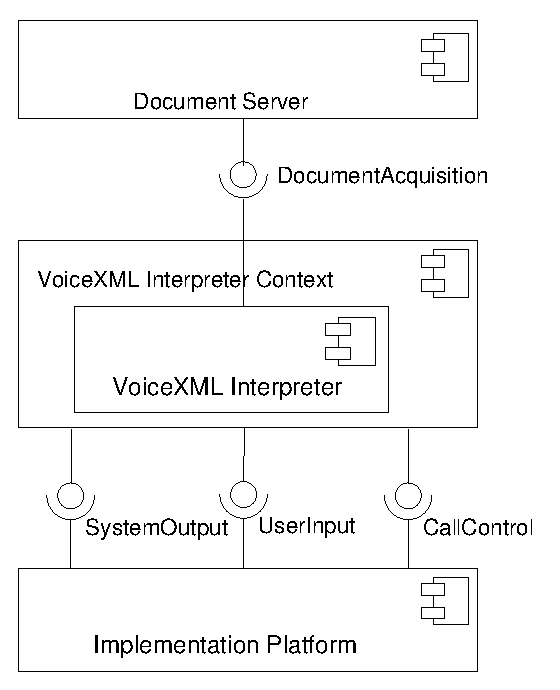
\includegraphics{overview.eps}
\end{center}

The architecture consists of three main components:
\begin{enumerate}
\item document server,
\item VoiceXML interpreter and
\item implementation platform.
\end{enumerate}

The first two parts can be used independent of each other. 
This offers the possibility
to use the VoiceXML document library for the JAVA programming language 
in conjunction with other VoiceXML interpreters,based on the open
industry standard VoiceXML.
At the implementation platform component side, the VoiceXML interpreter can be
used to process your VoiceXML documents, independent if you were using the 
VoiceXML document library, using hooks based on JSAPI and JTAPI.
This makes the interpreter vendor independent, as long these standards
are supported.

The components have a direct impact on the package structure, which is shown
in the following figure.

\begin{center}
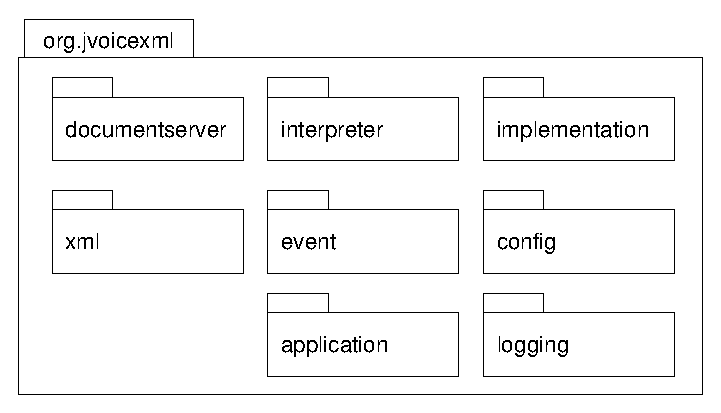
\includegraphics{package-org.jvoicexml.eps}
\end{center}

Each of the components named above has a
corresponding part as a package. 
\begin{description}
\item[org.jvoicexml.documentserver] Implementation of the document server,
\item[org.jvoicexml.interpreter] Implementation of the VoiceXML interpreter and
\item[org.jvoicexml.implementation] Implementation of the implementation 
platform.
\end{description}

Besides are some utility packages:
\begin{description}
\item[org.jvoicexml.application] Representation of applications.
\item[org.jvoicexml.config] Handle configuration issues.
\item[org.jvoicexml.logging] Handle logging issues.
\item[org.jvoicexml.xml] Enable parsing and creation of VoiceXML documents.
\item[org.jvoicexml.events] Define events that can be thrown by all of the 
other components and are caught by the center component 
\emph{VoiceXML Interpreter Context}.
\end{description}

The main package \texttt{org.jvoicexml} contains the classes which
serve as an entry point for VoiceXML interpretation.

\section{Detailed Component Description}
\label{sec:deta-comp-descr}

\subsection{Main Component}
\label{sec:main-component}

\subsubsection{Task of the Component}

The classes of this package serve as an entry point for VoiceXML
interpretation. This includes resource and session management.

\subsubsection{Structure of the Component}

The main component contains only two classes: \texttt{JVoiceXML} and 
\texttt{Session} which is shown in the following class diagram.

\begin{center}
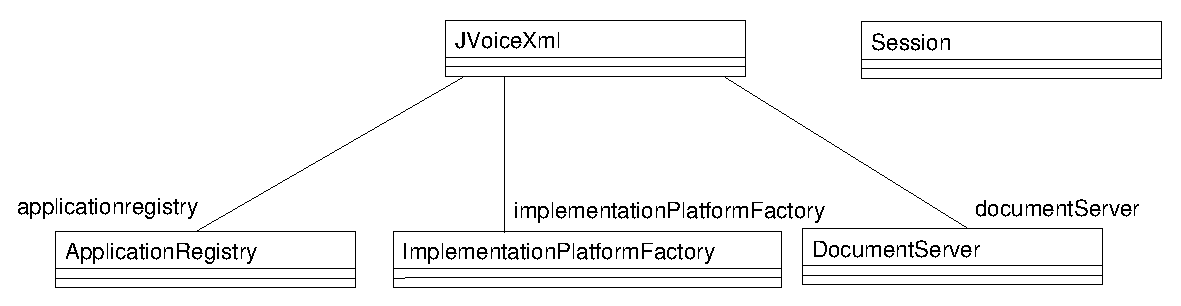
\includegraphics[scale=0.6]{class-main.eps}
\end{center}

\texttt{JVoiceXml} serves a a \texttt{Session} factory and is responsible
for resource management. 

\subsection{Document Server Component}
\label{sec:docum-serv-comp}

\subsubsection{Task of the Component}

This is the realization of the \emph{Document Server} component.

The main purpose of the \texttt{DocumentServer} is to process requests from a 
client application.

The document server evaluates the scheme of the incoming requests and
calls the appropriate \texttt{SchemeStrategy} to create VoiceXML
documents in response. Each document can be identified uniquely by
it's URI~\cite{w3.org:addressing}.

This implementation of a document server is only responsible for
evaluating the scheme selection of the corresponding document repository,
e.g. a web server.

\subsubsection{Structure of the Component}

As shown in the following class diagram, a \texttt{DocumentServer}
knows multiple \emph{SchemeStrategies}.

\begin{center}
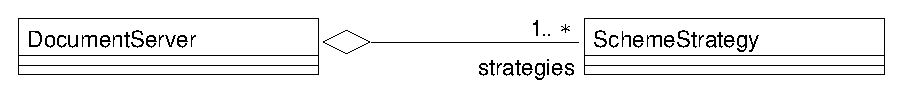
\includegraphics[scale=0.8]{class-documentserver.eps}
\end{center}

\subsubsection{Interfaces of the Component}

\subsection{VoiceXML Interpreter Component}
\label{sec:voic-interpr-comp}

\subsubsection{Task of the Component}

This is the realization of the 
\emph{VoiceXML Interpreter Context} and the \emph{VoiceXML Interpreter}
component. It processes VoiceXML documents retrieved from the
\texttt{DocumentServer}.

\subsubsection{Structure of the Component}

\begin{center}
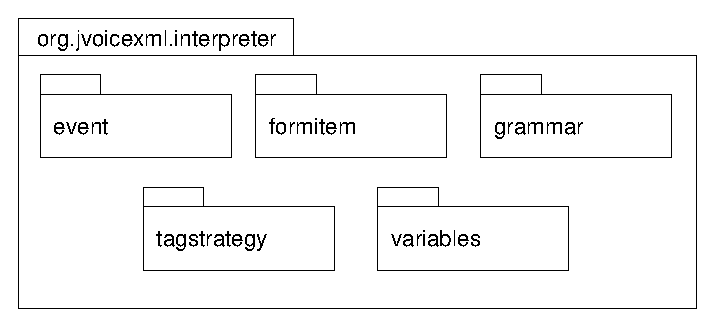
\includegraphics{package-org.jvoicexml.interpreter.eps}
\end{center}

\subsubsection{Interfaces of the Component}

\subsection{Implementation Platform Component}
\label{sec:impl-platf-comp}

\subsubsection{Task of the Component}

This is the realization of the \emph{Implementation Platform}
component.

\subsubsection{Structure of the Component}

The package structure of this component is shown in the following
package diagram.

\begin{center}
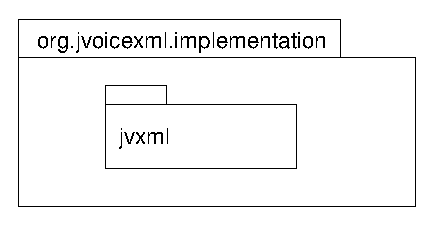
\includegraphics{package-org.jvoicexml.implementation.eps}
\end{center}

These packages have the following purpose:

\begin{description}
\item[org.jvoicexml.implementation] Core classes of the implementation
platform.
\item[org.jvoicexml.implementation.jvxml] Demo implementation of
an implementation platform.
\end{description}

The \texttt{ImplementationPlatformFactory} is a factory for
\texttt{Implementation\-Platform}s which are held in a pool.
This is currently not implemented, but will be realized as soon as possible.
Currently there is only one member in the pool.

\begin{center}
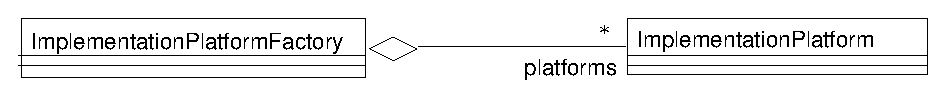
\includegraphics[scale=0.8]{class-implementationplatformfactory.eps}
\end{center}

The main class of the implementation platform component is 
\texttt{Implemen\-tat\-ion\-Plat\-form} which is held in a pool of 
implementation
platforms by the \texttt{Implementat\-ionPlat\-form\-Factory}. This means
that each session owns exactly one \texttt{Implemen\-tat\-ionPlat\-form}
object.

\begin{center}
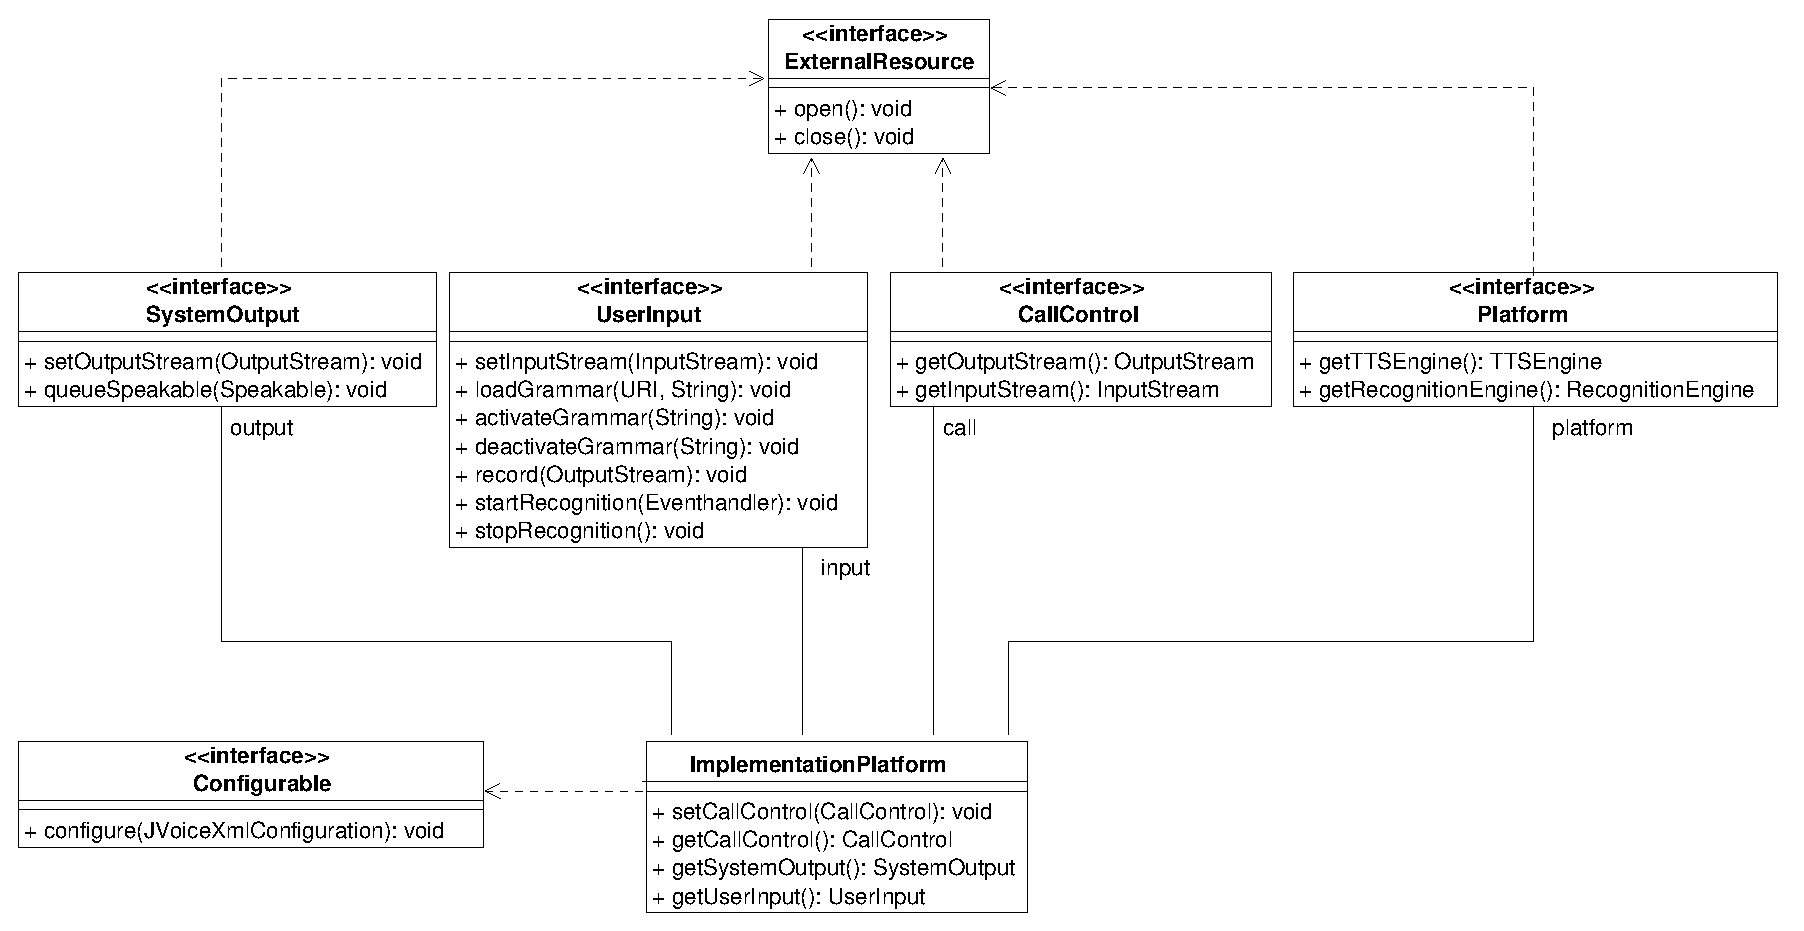
\includegraphics[scale=0.4]{class-implementation-implementationplatform.eps}
\end{center}

\subsubsection{Interfaces of the Component}

\subsection{Application Component}

\subsubsection{Task of the Component}

An \texttt{Application} is a set of documents sharing the same 
application root document.

Whenever the user interacts with a document in an application, its
application root document is also loaded. The application root document
remains loaded while the user is transitioning between other documents in the
same application, and it is unloaded when the user transitions to a document
that is not in the application. While it is loaded, the application root
document's variables are available to the other documents as application
variables, and its grammars remain active for the duration of the
application.

\subsubsection{Structure of the Component}

\begin{center}
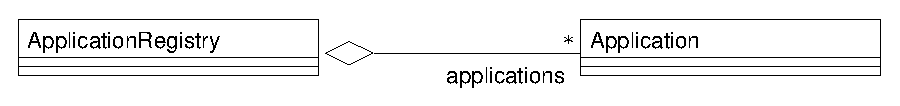
\includegraphics[scale=0.6]{class-application.eps}
\end{center}

\subsubsection{Interfaces of the Component}

\subsection{Configuration Component}
\label{sec:conf-comp}

\subsubsection{Task of the Component}

This component contains classes to allow for easy access to the configuration
files.

There is currently one configuration file called \emph{jvoicexml.xml}
which is expected to be in the root directory of the classpath.

\subsubsection{Structure of the Component}

The central instance of this component is the class
\texttt{JVoiceXmlConfiguration} which encapsulates access to the
configuration file.

All configurable objects must implement the \texttt{Configurable}
interface. Thus, the individual components are responsible for
evaluating the configuration file.

\subsubsection{Interfaces of the component}

\subsection{Logging Component}
\label{sec:logging-component}

\subsubsection{Task of the Component}

This component contains classes to handle logging mechanisms.

\subsubsection{Structure of the Component}

\subsubsection{Interfaces of the component}

\subsection{XML Component}
\label{sec:xml-component}

\subsubsection{Task of Component}

This package contains classes for easy creation and parsing of VoiceXML
documents.

VoiceXML is designed for creating audio dialogs that feature synthesized
speech, digitized audio, recognition of spoken and DTMF key input, recording
of spoken input, telephony and mixed initiative conversations. Its major goal
is to bring the advantages of web-based development and content delivery to
interactive voice response applications.

\subsubsection{Structure of the Component}

\begin{center}
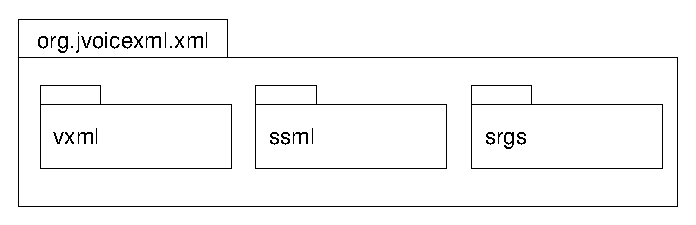
\includegraphics{package-org.jvoicexml.xml.eps}
\end{center}

\subsubsection{Interfaces of the Component}

\subsection{Event Component}
\label{sec:event-component}

\subsubsection{Task of the Component}

The \texttt{ImplementationPlatform} throws events when the user does not 
respond, doesn't respond in a way that the application understands, requests 
help, etc. The interpreter
throws events if it finds a semantic error in a VoiceXML document, or when it
encounters a \texttt{<throw>} element. Events are identified by
character strings.

\subsubsection{Structure of the Component}

Events are subdivided into plain events, things that happen normally, and
error events, abnormal occurrences.

This has a direct impact on the package structure.

\begin{center}
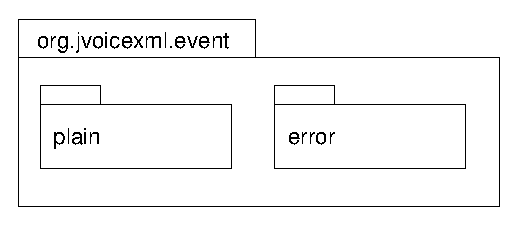
\includegraphics{package-org.jvoicexml.event.eps}
\end{center}

In addition, there are two basic event classes, which are derived from
a general \texttt{JVoiceXMLEvent}.

\begin{center}
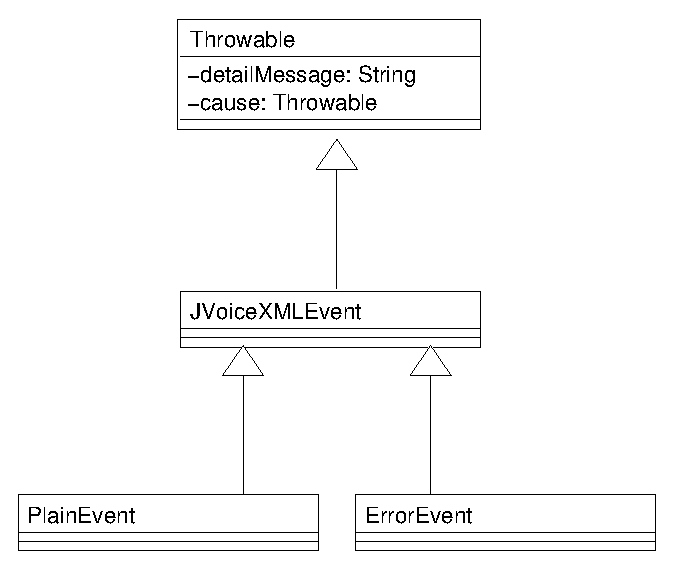
\includegraphics[scale=0.6]{class-event.eps}
\end{center}

\subsubsection{Interfaces of the Component}

\section{Detailed Module Description}
\label{sec:deta-module-descr}

\subsection{Module Resource Management of the main component}

\texttt{JVoiceXml} is the main object and is responsible to instantiate and
acquire all needed resources. It is implemented as the GoF's creational
pattern Singleton\cite{gamma:design_patterns}. References
can only be retrieved by calling it's static \texttt{getInstance()} method.

\begin{center}
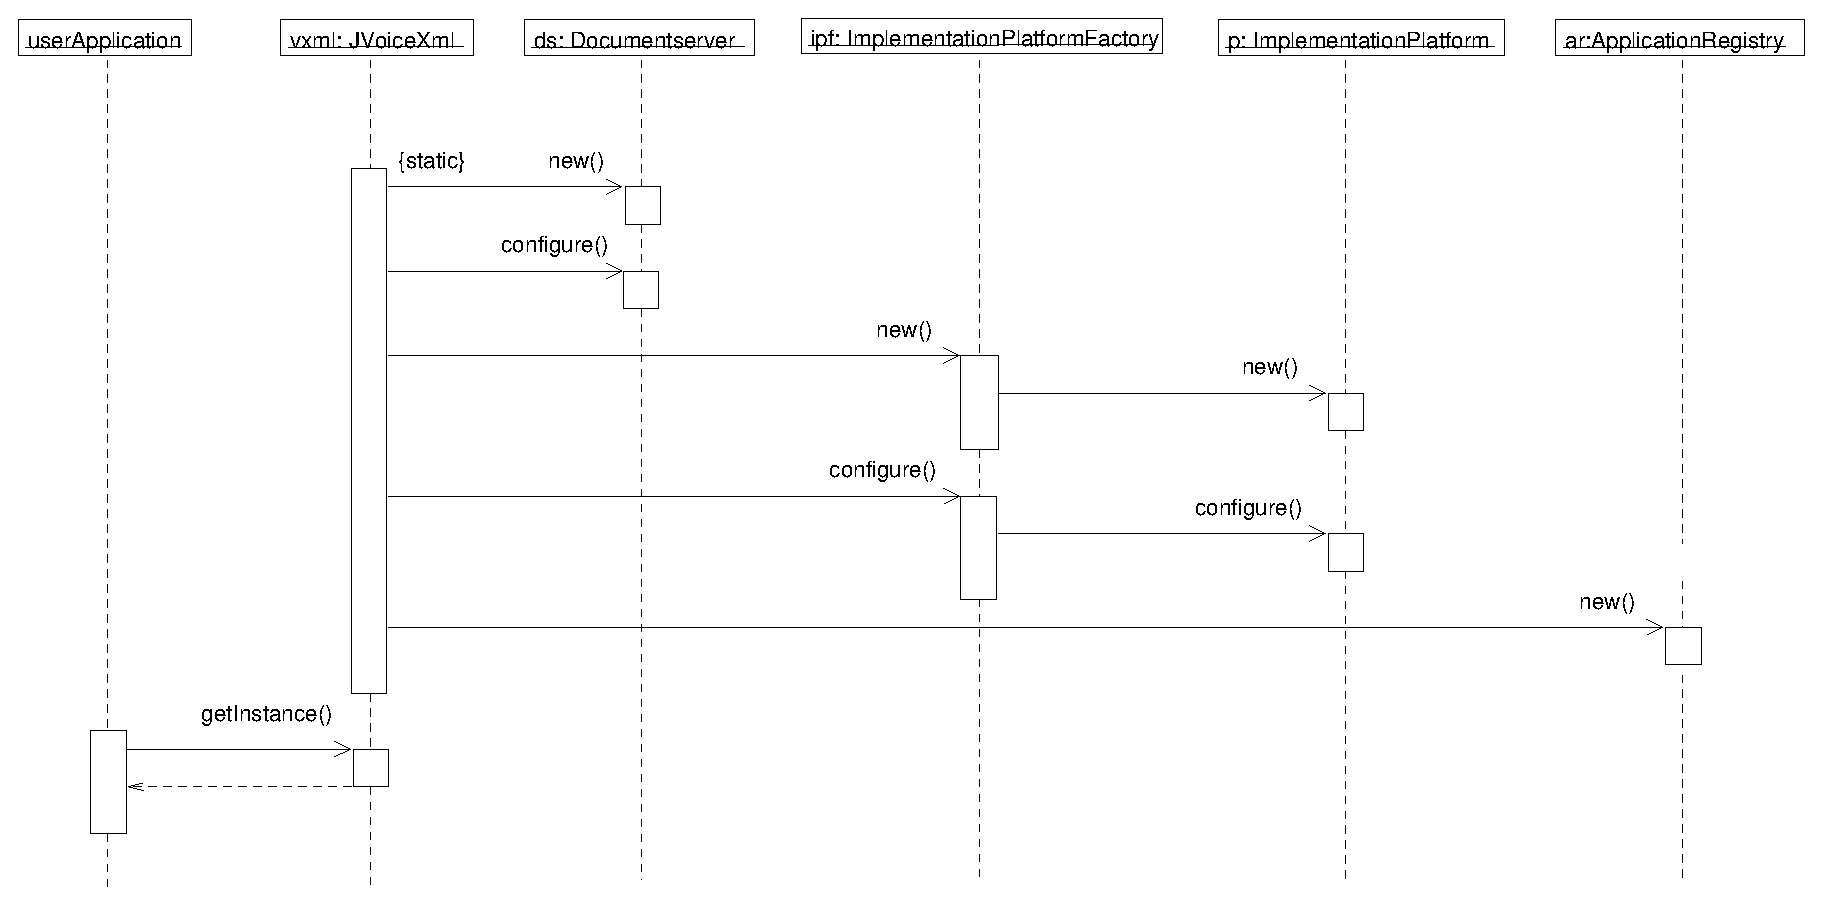
\includegraphics[scale=0.4]{seq-jvoicexml-startup.eps}
\end{center}

On startup this central object instantiates all needed resources:

\begin{itemize}
\item the implementation platform factory,
\item the document server and
\item the application registry.
\end{itemize}

It also offers methods to access the document server and the application
registry.

The implementation platform factory instantiates and configures all
resources related the platform, like \texttt{SystemOutput} and
\texttt{UserInput} as shown in the following sequence diagram.

\begin{center}
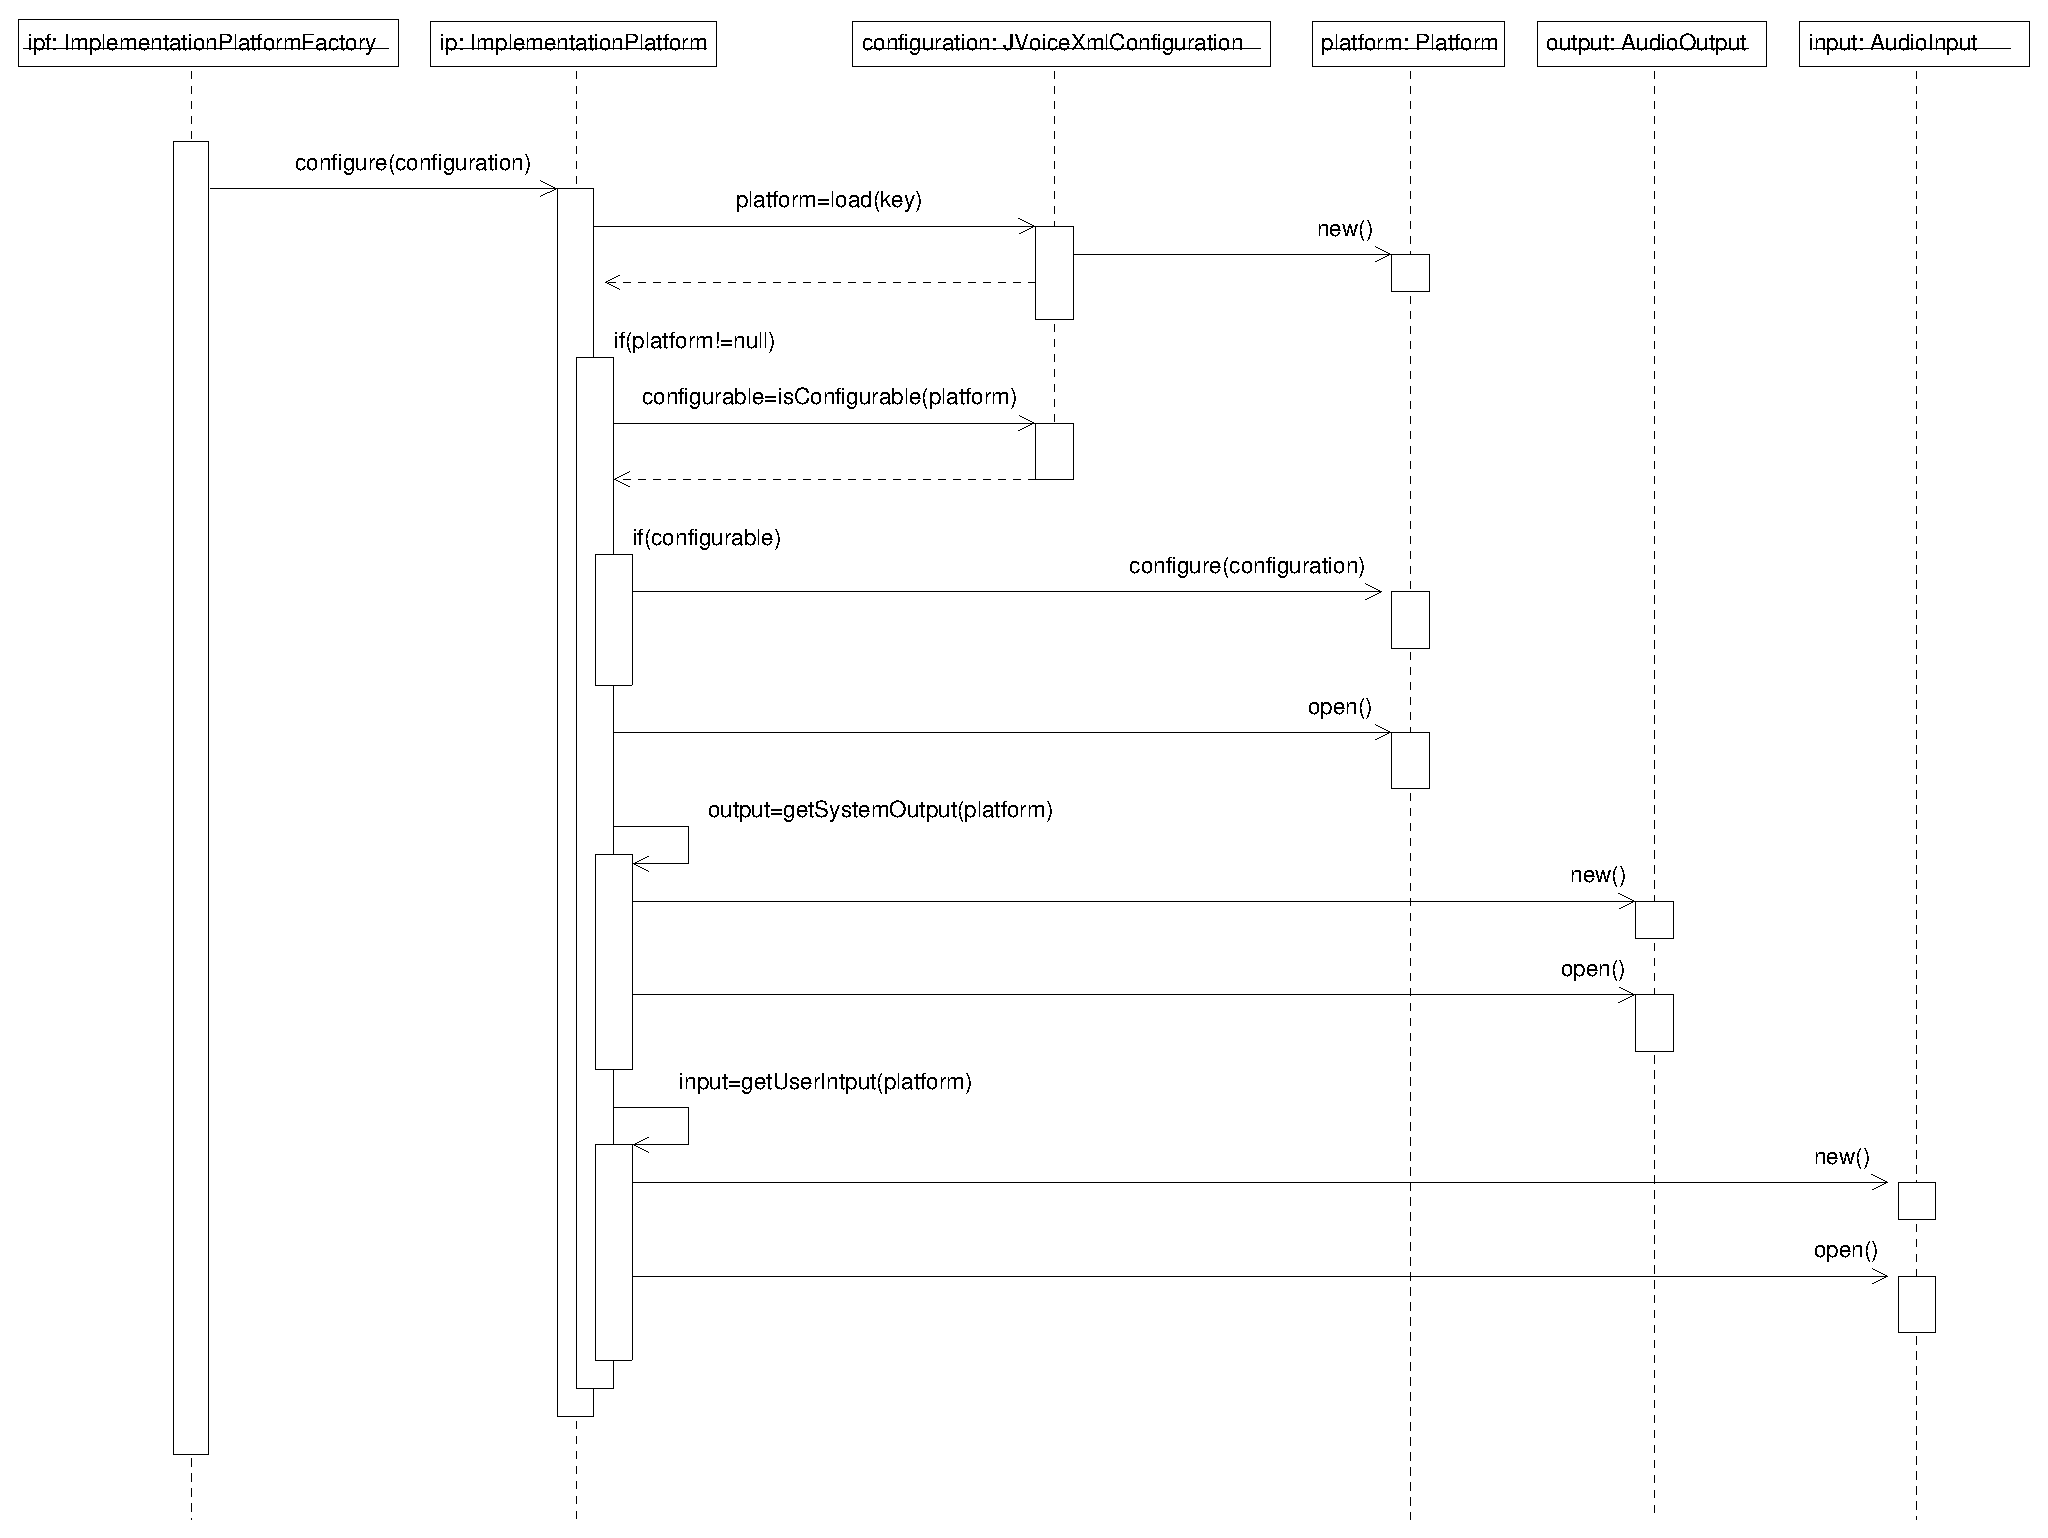
\includegraphics[scale=0.35]{seq-implementation.eps}
\end{center}

\subsection{Module Session management of the main component}

\texttt{JVoiceXml} is a \texttt{Session} factory\cite{gamma:design_patterns}. 
Sessions are the heart of a user session, while working with the VoiceXML 
interpreter.

The following sequence diagram shows, how a session is retrieved
from the main component.

\begin{center}
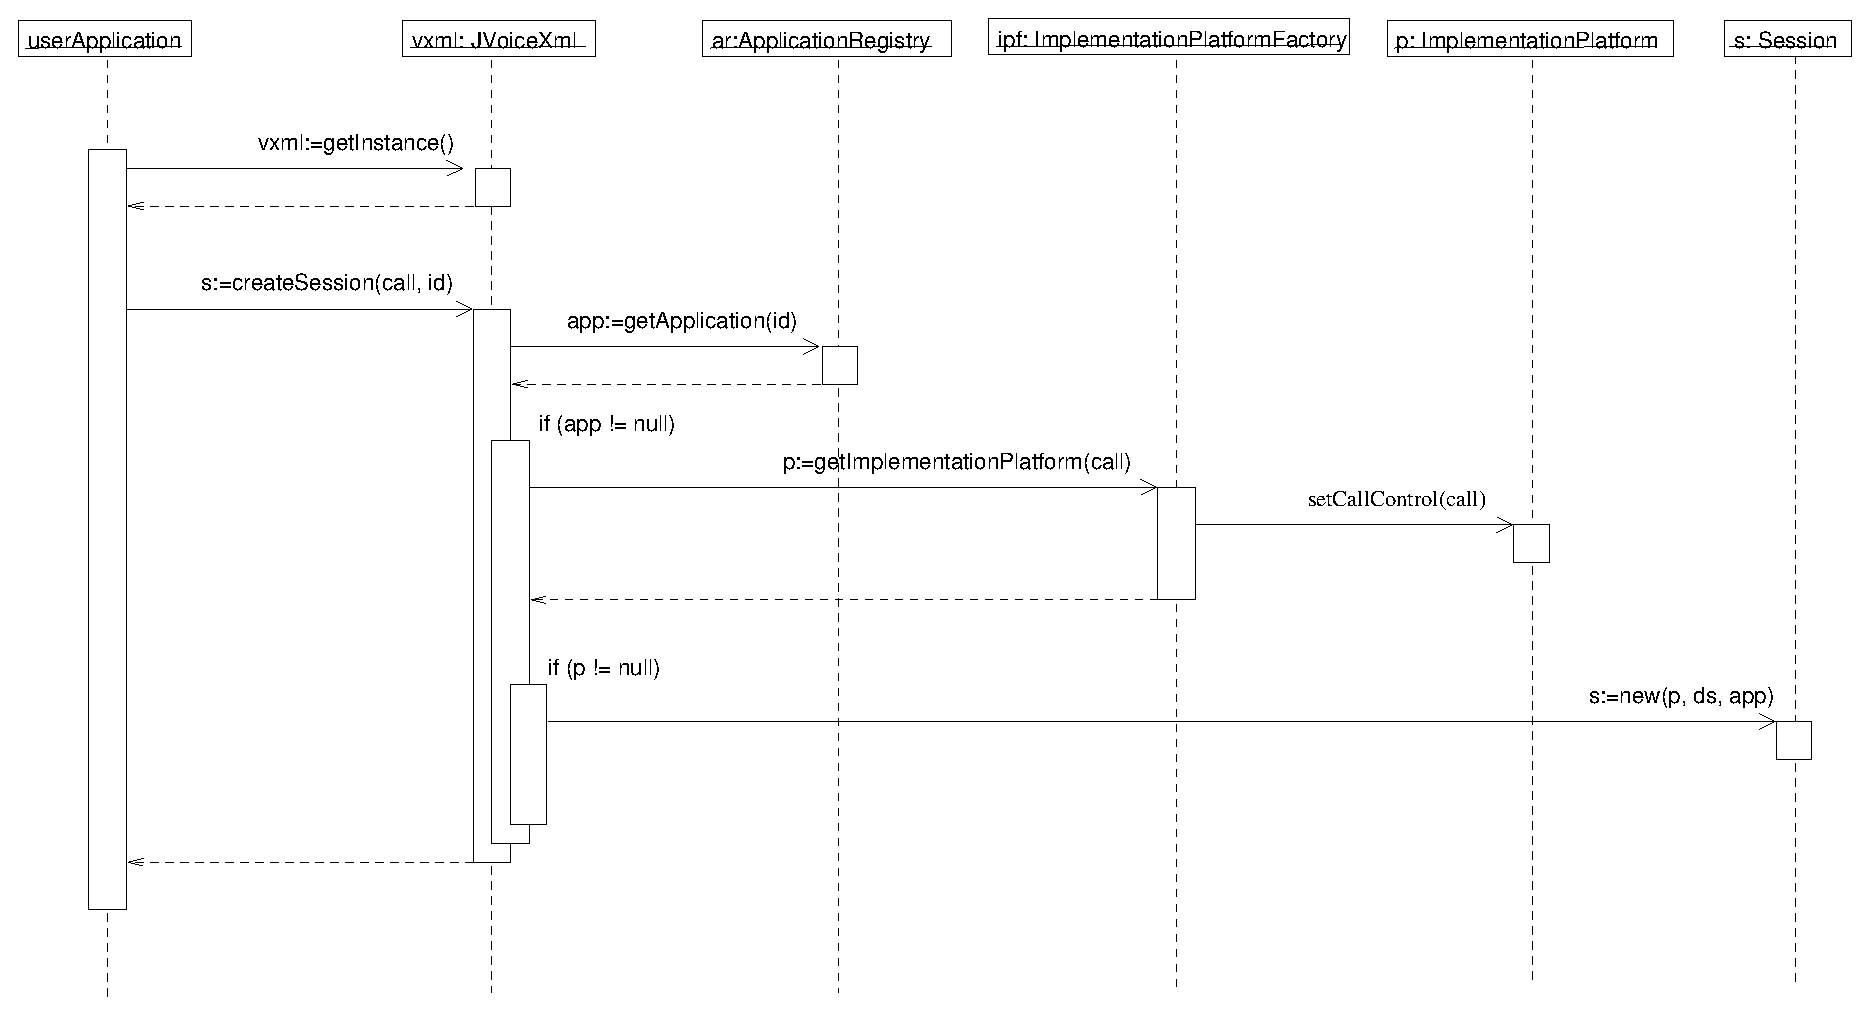
\includegraphics[scale=0.4]{seq-jvoicexml-sessionfactory.eps}
\end{center}

If the \texttt{Session} is not used any more, the allocated resources
can be returned by calling the \texttt{close()} method.

\begin{center}
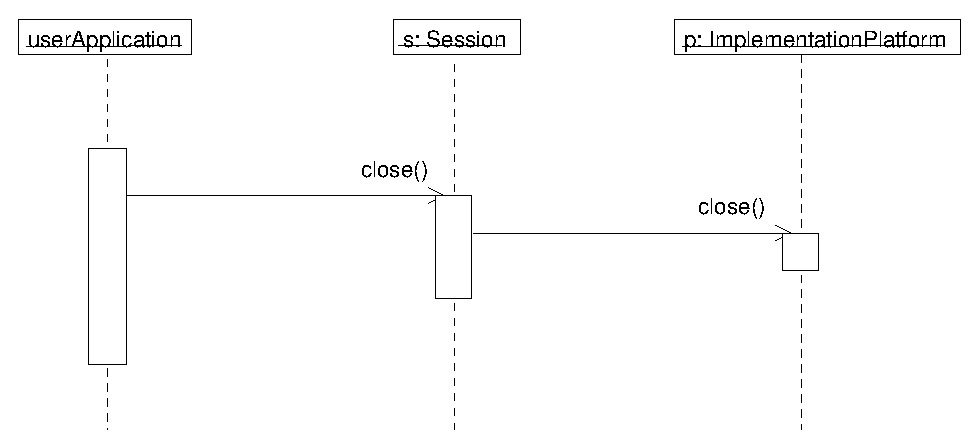
\includegraphics[scale=0.6]{seq-jvoicexml-sessionclose.eps}
\end{center}

\subsection{Module Document Retrieval of the Document Server component}
\label{sec:module-docum-serv}

The document server uses the strategy pattern~\cite{gamma:design_patterns} 
to process the different schemes.
Each instance of the \texttt{SchemeStrategy} interface knows how
to handle a specific URI scheme.

The anatomy of a call to the \texttt{DocumentServer} to retrieve a
document by it's URI is shown in the following sequence diagram.

\begin{center}
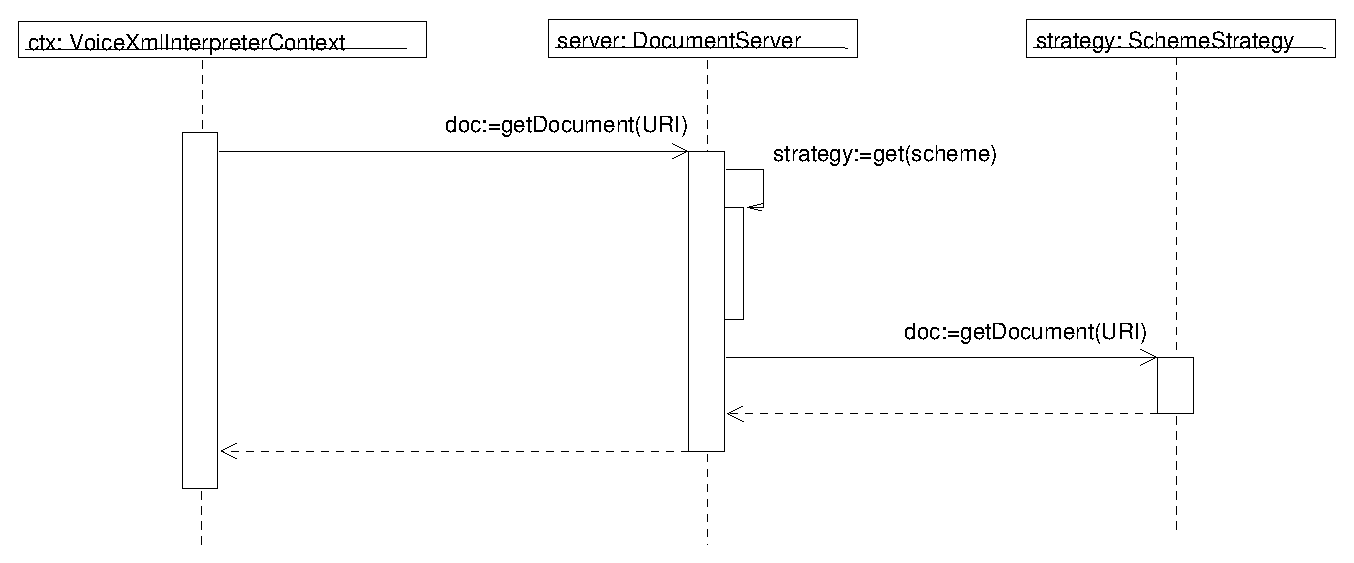
\includegraphics[scale=0.5]{seq-documentserver.eps}
\end{center}

\subsection{Module Form Interpretation Algorithm of the VoiceXML Interpreter 
component}
\label{sec:module-form-interpr}

The implementation of the \texttt{FormInterpretationAlgorithm} 
follows the description given in~\cite{w3.org:voicexml} section 2.1.6
and Appendix C.

The VoiceXML specification~\cite{w3.org:voicexml} names two main
functions of the form interpretation algorithm:
\begin{enumerate}
\item Initialization phase and
\item main loop.
\end{enumerate}

They are called from the \texttt{VoiceXmlInterpreter} as shown in the
following sequence diagram.

\begin{center}
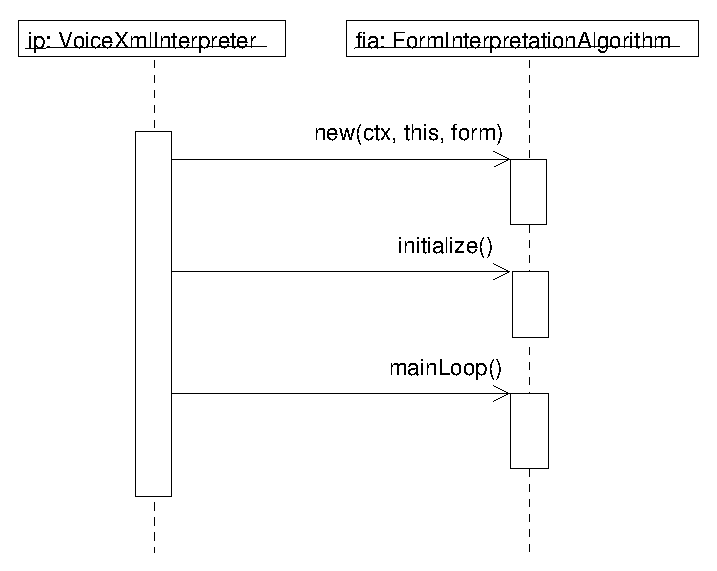
\includegraphics[scale=0.7]{seq-interpreter-fia.eps}
\end{center}

The \emph{Initialization phase} is called whenever a form is entered.
Internal prompt counter variables (in the form's dialog scope) are reset to 1.
Each variable (form-level \texttt{<var>} elements and form item variables) is 
initialized, in document order, to undefined or to the value of the relevant 
\texttt{expr} attribute.

This is implemented with the help of \texttt{InitializationStrategy}s.
When the \texttt{ForminterpretationAlgorithm} initialization comes to a 
VoiceXML tag, it asks the \texttt{InitializationStrategyFactory} for a strategy
how to initialize the current node. If a matching strategy was found, the
\texttt{execute()} method of the returned \texttt{InitializationStrategy}
is called, as shown in the following sequence diagram:

\begin{center}
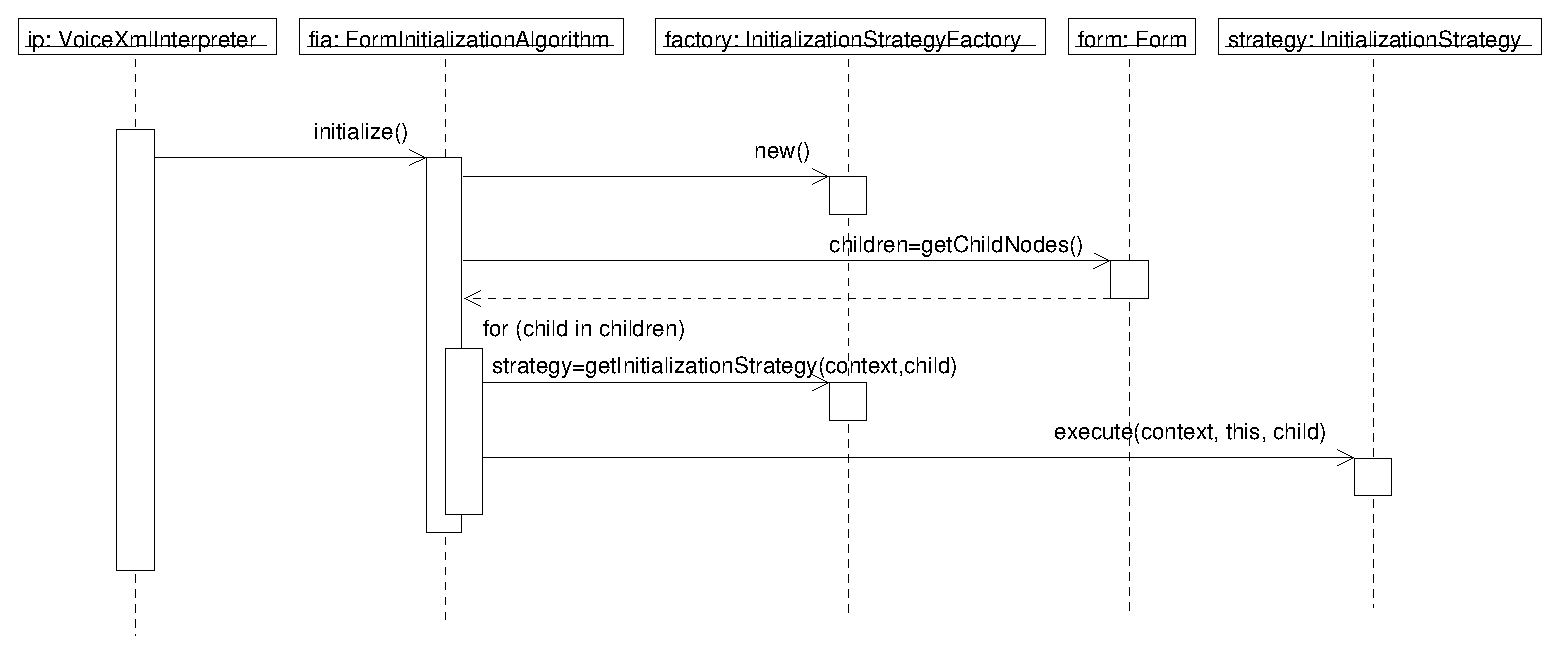
\includegraphics[scale=0.45]{seq-interpreter-fia-initialize.eps}
\end{center}

The \emph{main loop} of the FIA, the \textbf{f}orm \textbf{i}nterpretation
\textbf{a}lgorithm, has three phases:

\begin{description}
\item[select phase] the next unfilled form item is selected for visiting.
\item[collect phase] the selected form item is visited, which prompts the user
for input, enables the appropriate grammars, and then waits for and collects 
an input (such as a spoken phrase or DTMF key presses) or an event 
(such as a request for help or a no input timeout).
\item[process phase] an input is processed by filling form items and executing
\texttt{<filled>} elements to perform actions such as input validation.
An event is processed by executing the appropriate event handler for that 
event type.
\end{description}

\begin{center}
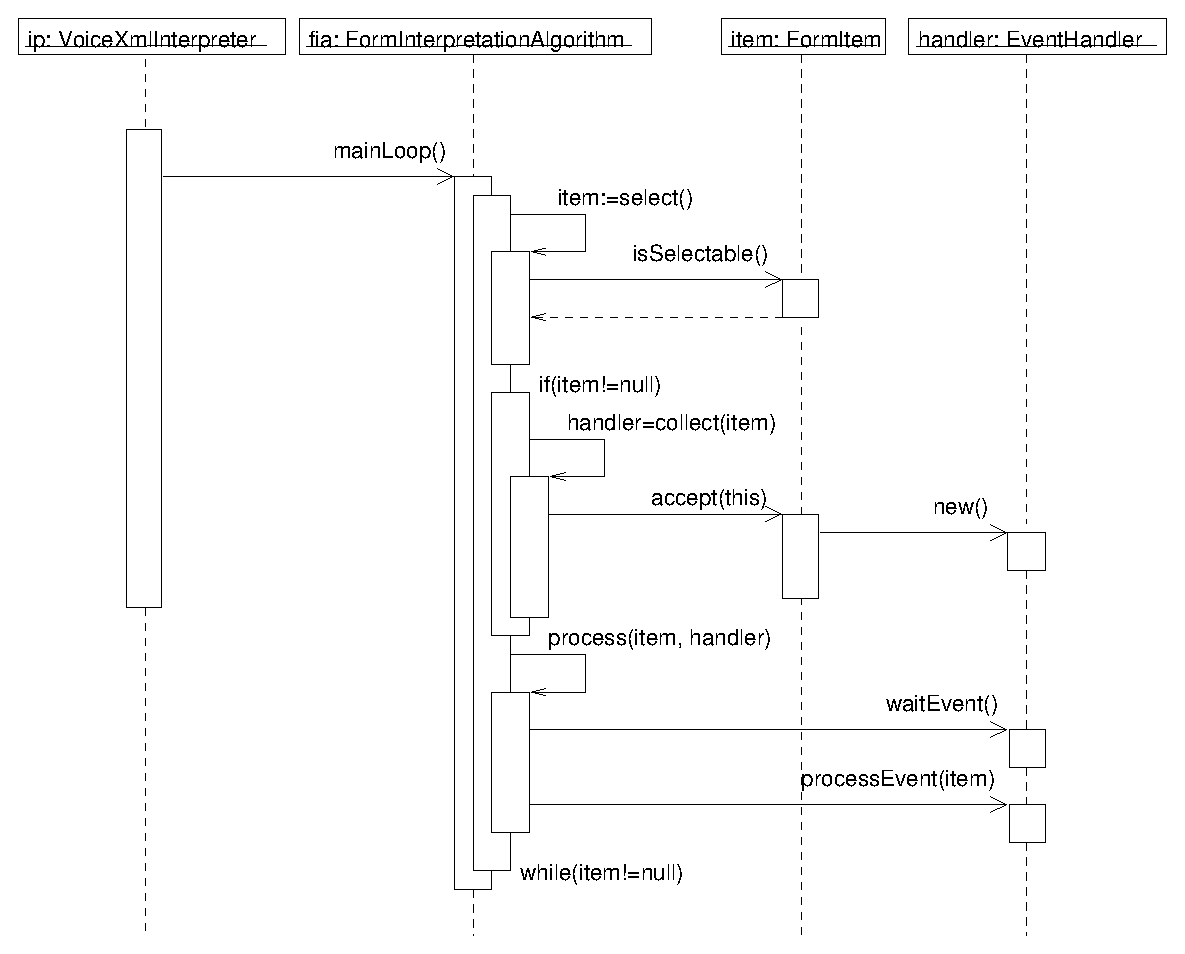
\includegraphics[scale=0.6]{seq-interpreter-fia-mainloop.eps}
\end{center}

The processing of the \texttt{FormItem}s in the collect phase
is implemented using the \emph{Visitor Pattern}.
The different kinds of form items, as described in section 2.1.2 
of~\cite{w3.org:voicexml} have their expression in subclassing the
\texttt{FormItem} as shown in the following class diagram.

\begin{center}
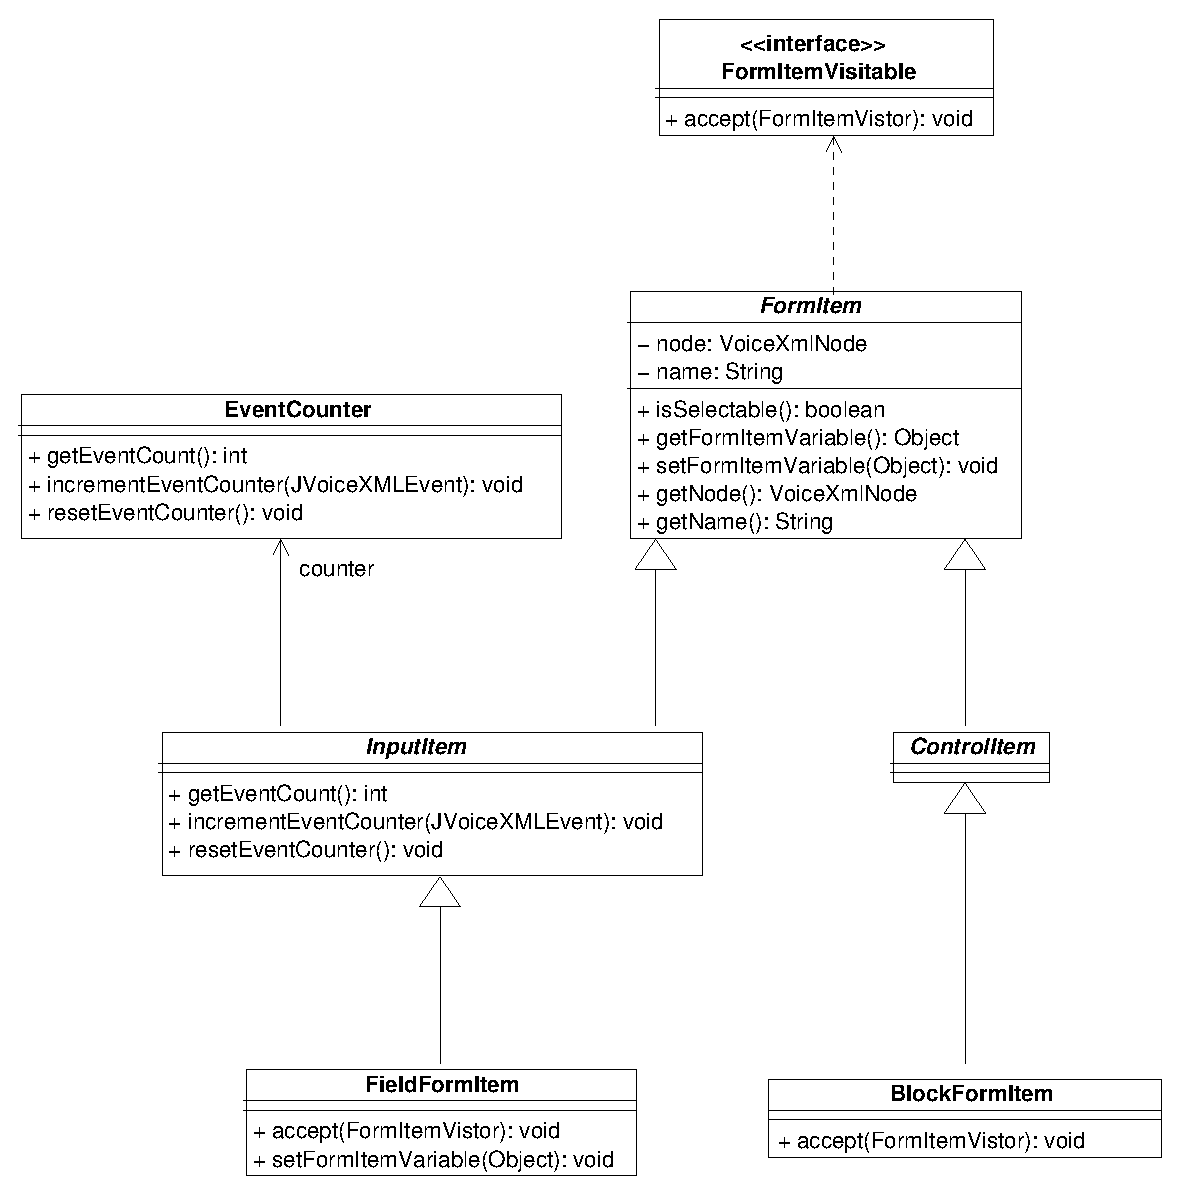
\includegraphics[scale=0.5]{class-interpreter-formitem.eps}
\end{center}

An overview, how the visitor is implemented is given in the following
class diagram.

\begin{center}
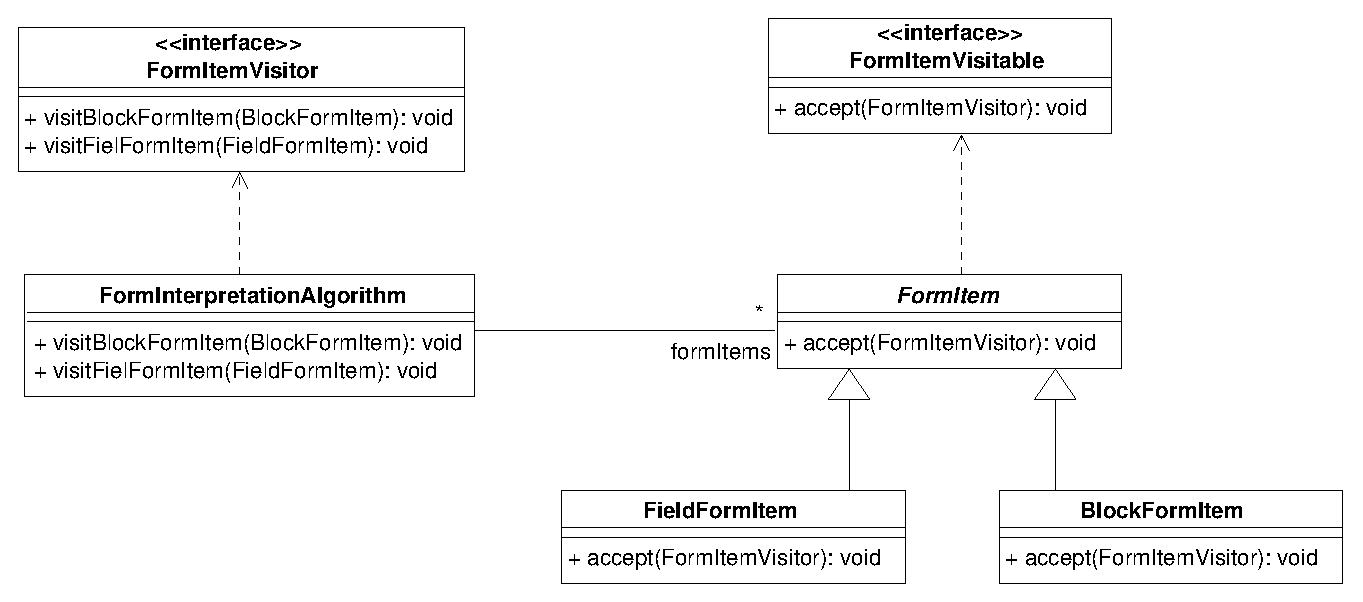
\includegraphics[scale=0.5]{class-interpreter-visitor.eps}
\end{center}

\subsection{Module ImplementationPlatform of the implementation platform 
component}


\subsection{Module VarRegistry of the VoiceXML Interpreter component}
\label{sec:module-varr-voic}

\subsection{Module Grammar Handler of the 
VoiceXML Interpreter component}

\subsection{Module ApplicationRegistry of the application component}

Registry for all known applications. All applications are identified
uniquely by their id.

The application registry allows for easy access to an application,
if only the id of the application is known. This may be used e.g. to
create a simple mapping from a a telephone line to the URI of the
application's root document.


\section*{Document history}

\begin{tabular}{|l|p{5cm}|l|l|}
\hline
\textbf{Version} & \textbf{Comment} & \textbf{Responsible} & \textbf{Date} \\
\hline
\hline
0.0.1 & Initial Release & Dirk Schnelle & 09/13/2005 \\
\hline
0.0.2 & Added application component & Dirk Schnelle & 09/18/2005 \\
\hline
0.0.3 & Initial content of FIA & Dirk Schnelle & 09/22/2005 \\
\hline
0.0.4 & Initial content of implementation platform & Dirk Schnelle & 09/22/2005 \\
\hline
0.0.5 & Added process phase to FIA, Initial content of logging component & 
Dirk Schnelle & 10/25/2005 \\
\hline
\end{tabular}

\bibliography{architecture}
\bibliographystyle{plain}

\end{document}





% LocalWords:  JVoiceXML VoiceXML API's JSAPI JTAPI SourceForge config xml org
% LocalWords:  SchemeStrategy ApplicationRegistry VarRegistry Schnelle GoF's
% LocalWords:  DocumentServer SchemeStrategies jvoicexml JVoiceXml getInstance
% LocalWords:  creational DTMF ImplementationPlatform JVoiceXMLEvent peech API
% LocalWords:  elephony FormInterpretationAlgorithm VoiceXmlInterpreter expr
% LocalWords:  FIA orm nterpretation lgorithm FormItem subclassing Implemen
% LocalWords:  ImplementationPlatformFactory Implementat ionPlat classpath
% LocalWords:  JVoiceXmlConfiguration SystemOutput UserInput
% LocalWords:  InitializationStrategy ForminterpretationAlgorithm
% LocalWords:  InitializationStrategyFactory
